 \documentclass[journal,10pt,twocolumn]{article}
\usepackage{graphicx, float}
\usepackage[margin=0.5in]{geometry}
\usepackage{amsmath, bm}
\usepackage{array}
\usepackage{booktabs}

\providecommand{\norm}[1]{\left\lVert#1\right\rVert}
\let\vec\mathbf
\newcommand{\myvec}[1]{\ensuremath{\begin{pmatrix}#1\end{pmatrix}}}
\newcommand{\mydet}[1]{\ensuremath{\begin{vmatrix}#1\end{vmatrix}}}

\title{\textbf{Circle Assignment}}
\author{Pallavarapu Sravan kumar}
\date{September 2022}

\begin{document}

\maketitle
\paragraph{\textit{\large Problem Statement} - In Figure 1. A,B,C are the three points with centre O such that $\angle$BOC=30$^\circ$ and $\angle$AOB=60$^\circ$.If D is a point on the circle other than the arc ABC,find $\angle$ADC}
\section*{\large Solution}
\begin{figure}[H]
\centering
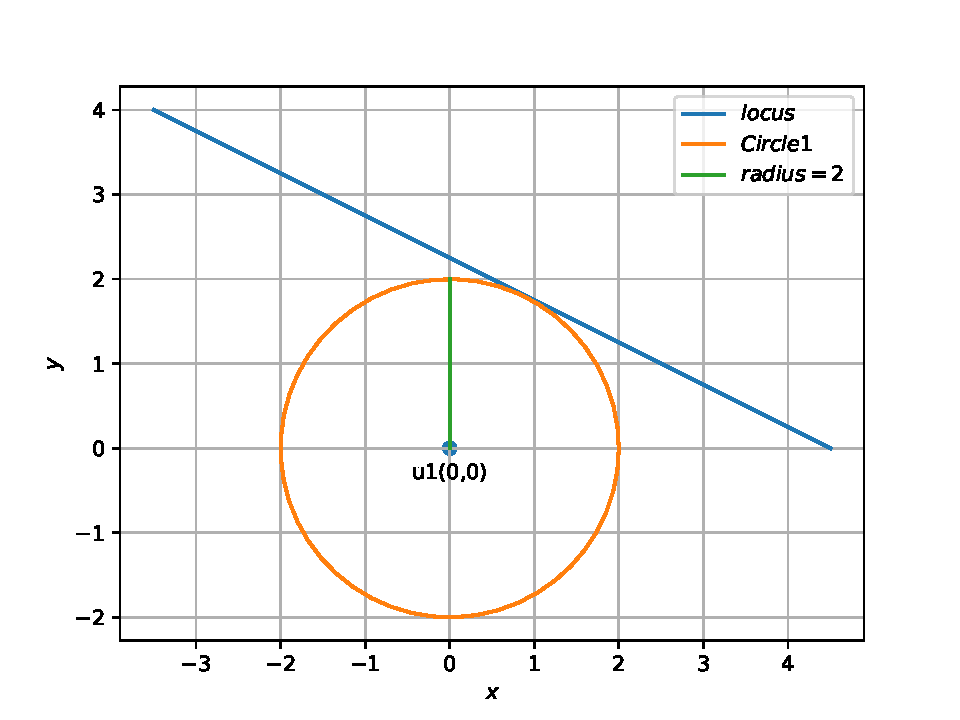
\includegraphics[width=1\columnwidth]{CoordGeo/circle1.pdf}
\caption{}
\end{figure}

\section*{\large Construction}



The input parameters are the lengths



\begin{table}[htbp]
 \begin{center}
    \begin{tabular}{|l|c|c|c|c|c|c} \hline \textbf{Symbol}
  & \textbf{value} & \textbf{Description} \\
 \hline
O & & centre \\ \hline
$\angle$BOC &30$^\circ$ & Angle between vectors B and C  \\ \hline
$\angle$AOB&60$^\circ$&Angle between vectors A and B\\
	\hline
	$\angle$ADC&??&Angle between vectors A and C \\
	\hline
\end{tabular}   
\end{center}
\caption{\label{table:dummytable} }
\end{table}

\vspace*{10mm}

\section*{\large Assumptions}
Let P be a point on the circle such that by expandig OC upto P we get diameter POC.



To find $\angle$ADC let the circle be unit circle and diameter POC on x axis.
\vspace*{3mm}

Take three points C,A,D  and $\alpha$,$\beta$,$\gamma$ be three angles made by the points C,A,D with respect to diameter POC.
\vspace*{3mm}

From the Figure 2:
\begin{equation}
\vec{\alpha} = \vec{\angle POC}= 180^\circ, 
\vec{\beta} = \vec{\angle POA} = 90^\circ,
\vec{\gamma} = \vec{\angle POD}
\end{equation}
 
\section*{Proof:}
From assumptions the vector points C,A,D be
\begin{eqnarray}
	\vec{C} = \myvec{cos\alpha\\sin\alpha},
	\vec{A} = \myvec{cos\beta\\sin\beta},
	\vec{D} = \myvec{cos\gamma\\sin\gamma}
\end{eqnarray}

Let AC be the chord that subtends angles at the center O and at point D. The cosine of the angle subtended at point D is given by
\begin{align}
	cos(\angle ADC) = \frac{(A-D)^T(C-D)}{\norm{A-D}\norm{C-D}}
	\label{pf2-eq-1}
\end{align}

Where
 \begin{eqnarray}
	\vec{A-D} = \myvec{cos\beta - cos\gamma\\sin\beta - sin\gamma},
	\vec{C-D} = \myvec{cos\alpha - cos\gamma\\sin\alpha - sin\gamma}
\end{eqnarray}
 

\begin{eqnarray*}
	(A-D)^T(C-D)=\myvec{cos\beta - cos\gamma  sin\beta - sin\gamma}
	\myvec{cos\alpha - cos\gamma\\sin\alpha - sin\gamma}
\end{eqnarray*}

\begin{multline*}
	= (\cos\alpha-\cos\gamma)(\cos\beta-\cos\gamma)+(\sin\alpha-\sin\beta)(\sin\beta-\sin\gamma)
\end{multline*}

\begin{multline*}
	= -2\sin\frac{\alpha-\gamma}2\sin\frac{\alpha+\gamma}2 \cdot(-2)\sin\frac{\beta-\gamma}2\sin\frac{\beta+\gamma}2 \\\quad+ 2\cos\frac{\alpha+\gamma}2\sin\frac{\alpha-\gamma}2 \cdot 2\cos\frac{\beta+\gamma}2\sin\frac{\beta-\gamma}2
\end{multline*}
\begin{multline*}
	= 4\sin\frac{\alpha-\gamma}2\sin\frac{\beta-\gamma}2(\sin\frac{\alpha+\gamma}2\sin\frac{\beta+\gamma}2+\\
	\cos\frac{\alpha+\gamma}2\cos\frac{\beta+\gamma}2)
\end{multline*}
\begin{align*}
	= 4\sin\frac{\alpha-\gamma}2\sin\frac{\beta-\gamma}2\cos\left(\frac{\alpha+\gamma}2-\frac{\beta+\gamma}2\right)
\end{align*}
\begin{align}
	= 4\sin\frac{\alpha-\gamma}2\sin\frac{\beta-\gamma}2\cos\frac{\alpha-\beta}2
	\label{pf2-eq-2}
\end{align}

\begin{multline*}
	\norm{A-D}^2\norm{C-D}^2 = ((\cos\alpha-\cos\gamma)^2+(\sin\alpha-\sin\gamma)^2)\\
	((\cos\beta-\cos\gamma)^2+(\sin\beta-\sin\gamma)^2)
\end{multline*}
\begin{multline*}
	= (2-2\cos\alpha\cos\gamma - 2\sin\alpha\sin\gamma)(2-\\
	2\cos\beta\cos\gamma - 2\sin\beta\sin\gamma)
\end{multline*}
\begin{align*}
	&= 4(1-\cos(\alpha-\gamma))(1-\cos(\beta-\gamma))\\
	&= 4\cdot 2\sin^2\frac{\alpha-\gamma}2\cdot 2\sin^2\frac{\beta-\gamma}2
\end{align*}
\begin{align*}
	&= 16 \sin^2\frac{\alpha-\gamma}2\sin^2\frac{\beta-\gamma}2
\end{align*}
\begin{align}
 \norm{A-D}\norm{C-D} = 4 \sin\frac{\alpha-\gamma}2\sin\frac{\beta-\gamma}2
	\label{pf2-eq-3}
\end{align}

Substituting (\ref{pf2-eq-2}) and (\ref{pf2-eq-3}) in (\ref{pf2-eq-1}),
\begin{multline*}
	cos(\angle ADC) = \frac{4sin\frac{\alpha-\gamma}{2}sin\frac{\beta-\gamma}{2}cos\frac{\alpha-\beta}{2}}{4 \sin\frac{\alpha-\gamma}2\sin\frac{\beta-\gamma}2}
\end{multline*}
\begin{equation}
cos(\angle ADC) = cos\frac{\alpha-\beta}{2}
\label{pf2-eq-4}
\end{equation}
\vspace*{5mm}
By substituting $\alpha$ and $\beta$ values in (\ref{pf2-eq-4})
\begin{equation*}
\angle ADC = \frac{\alpha-\beta}{2}=\frac{(180^\circ - 90^\circ )}{2}=45^\circ
\end{equation*}
















 
\end{document}
